\section{Results}

The various algorithms have been timed on CPU and runtimes have been plotted against sequences length in log2-log2 scale. Algorithms that scale linearly with sequence length have a slope of 1, while algorithms that scale quadratically with sequence length have a slope of 2. The Figure \ref{fig:RPE_timings}, shows the timings of the $A_{rel}$ matrix calculation. On Figure \ref{fig:kernelized_attention_timings} the kernelized attention algorithms have been timed. We can observe that although our algorithm for masked attention has a linear complexity, our linear algorithm is still often slower than the quadratic complexity algorithm. The bottleneck in our implementation was the cumulated sum operation over the $Unrolled$ tensor, which was surprisingly slow. A CUDA implemented operation might still be beneficial for this particular algorithm, also there might still be room for optimization in our implementation. Finally Figure \ref{fig:multihead_attention_timings} shows the timings of the vanilla multi-head attention compared to our proposed multi-head kernelized attention calculated with dynamically chosen algorithms.

\begin{figure}
	\center
	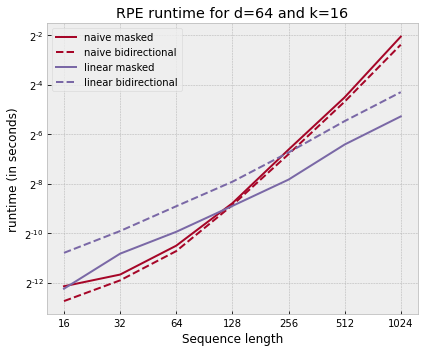
\includegraphics[width=0.9\linewidth]{images/runtimes_RPE.png}
	\caption{$A_{rel}$ calculation runtimes on CPU for $d=256$ and $k=10$}
	\label{fig:RPE_timings}
\end{figure}

\begin{figure}
	\center
	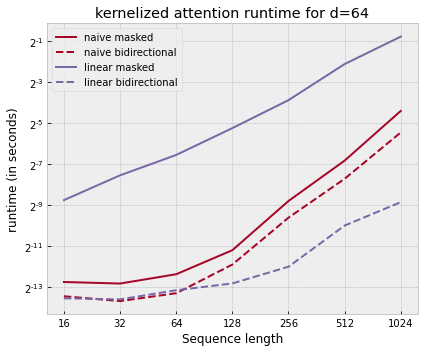
\includegraphics[width=0.9\linewidth]{images/runtimes_KA.png}
	\caption{kernelized attention runtimes on CPU for $d=256$}
	\label{fig:kernelized_attention_timings}
\end{figure}

\begin{figure}
	\center
	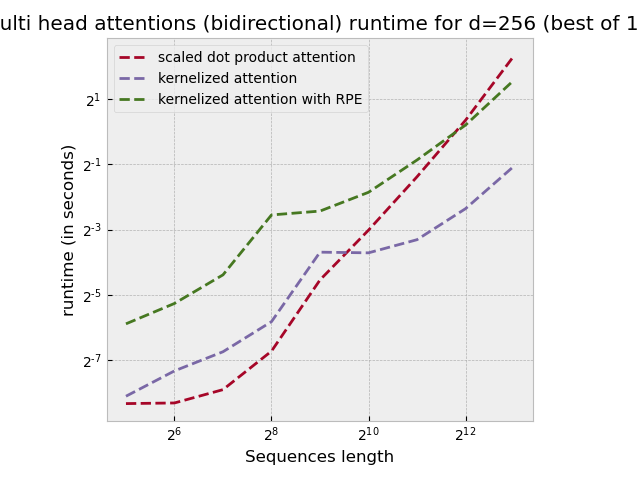
\includegraphics[width=0.9\linewidth]{images/runtimes_MHA.png}
	\caption{multi-head attention runtimes on CPU (bidirectional attentions only)}
	\label{fig:multihead_attention_timings}
\end{figure}

\endinput
